\documentclass[12pt,a4paper]{article} %hoja A4 y tamño de letra 12pt
\usepackage{setspace}
\onehalfspacing %interlineado 1,5 (no parece el mismo de Word pero es Word el que hace mal eso, este es el posta)
\usepackage[spanish,es-tabla]{babel} %idioma español y "tabla" en lugar de "cuadro"
\usepackage{fontspec}
\setmainfont{Calibri}
%\setmainfont{Times New Roman} %solamente para la primera entrega
%\newfontfamily\myfont{Calibri} %solamente para la primera entrega
\usepackage{datetime}
\usepackage{fancyhdr} %para alinear números de página a la derecha
\usepackage{lipsum}
\renewcommand{\headrulewidth}{0pt}%
\newdateformat{monthyeardate}{
  \monthnamespanish[\THEMONTH]  \THEYEAR}  \makeatletter	
\renewcommand{\monthnamespanish}[1][\month]{%
  \@orgargctr=#1\relax
  \ifcase\@orgargctr
    \PackageError{datetime}{Invalid Month number \the\@orgargctr}{%
      Month numbers should go from 1 to 12}%
    \or Enero%
    \or Febrero%
    \or Marzo%
    \or Abril%
    \or Mayo%
    \or Junio%
    \or Julio%
    \or Agosto%
    \or Septiembre%
    \or Octubre%
    \or Noviembre%
    \or Diciembre%
    \else \PackageError{datetime}{Invalid Month number \the\@orgargctr}{%
      Month numbers should go from 1 to 12}%
  \fi}
\makeatother
\usepackage{amsmath,amsfonts,amssymb}
\usepackage{graphicx} %para figuras
\usepackage[font=footnotesize]{caption} %descripciones de tablas/figuras en 10pt
\graphicspath{ {imagenes/} } %carpeta donde guardar imágenes
\usepackage{luatodonotes}
\setlength{\marginparwidth}{2 cm}
\usepackage[left=3cm,right=2.5cm,top=2.5cm,bottom=2.5cm]{geometry} %márgenes
%\usepackage[sorting=none,maxbibnames=99,isbn=false,doi=false,eprint=false,giveninits=true]{biblatex}
\usepackage[
backend=biber,
sorting=none,
style=numeric-comp
]{biblatex} %referencias
\renewbibmacro{in:}{}
\DeclareNameAlias{default}{last-first}
\addbibresource{referencias.bib} %añade archivo de referencias
\usepackage{tikz}
\usetikzlibrary{calc}
\usetikzlibrary{babel}
\usepackage{titlesec}
\titleformat{\section}{\normalfont\fontsize{16}{19}\bfseries}{\thesection.}{0.5em}{\MakeUppercase} %formato de título
\titleformat{\subsection}{\normalfont\fontsize{14}{16}\bfseries}{\thesubsection.}{0.5em}{\MakeUppercase} %formato de subtítulo
\titleformat{\subsubsection}{\normalfont\fontsize{14}{16}}{\thesubsection.}{0.5em}{} %formato de sub-subtítulo
\let\labelitemi\labelitemii

%Esto se modifica como quieran:
\author{Autor}
\title{Título}
  % mete el contenido del archivo head.tex como preámbulo

\begin{document}  % acá empieza la diversión
\pagenumbering{gobble}
\begin{titlepage}
	%\myfont %solamente para la primera entrega
	\begin{tikzpicture}[remember picture, overlay]
  	\draw[line width = 1pt] ($(current page.north west) + (1cm,-1cm)$) rectangle ($(current page.south east) + (-1cm,2cm)$);
	\end{tikzpicture}
    \begin{center}
	   	   
	   
\includegraphics[width=0.8\textwidth]{logo} 
	          
        \vspace*{1cm}
        \fontsize{18pt}{22pt}\selectfont
        \textbf{INGENIERÍA DE SONIDO}
               
        \vspace{4cm}
        \fontsize{22pt}{26pt}\selectfont
        \textbf{Título\dag}
        
        \vspace{3cm}
        \fontsize{18pt}{22pt}\selectfont
        \textbf{Autor: Nombre Apellido}
        
        \fontsize{16pt}{16pt}\selectfont
        \textbf{Tutor: Nombre Apellido}\par
        \textbf{Co-tutor: Nombre Apellido} %se puede sacar si no hay co-tutor
        
        \vspace{2cm}
        \fontsize{12pt}{14pt}\selectfont
        \textbf{(\dag) Tesis para optar por el título de ingeniero/a de Sonido}
        
        \vspace{1cm}
        
      
        
        \fontsize{14pt}{17pt}\selectfont
        \monthyeardate\today
        
    \end{center}
\end{titlepage}
%\tableofcontents % índice (comentado por ahora)
%\section{Resumen/Abstract} % resumen (comentado por ahora)
\begin{center}
	\pagenumbering{arabic}
	\fontsize{14pt}{17pt}\selectfont
	\textbf{Título de la Investigación}
\end{center}
\begin{flushleft} 
	\fontsize{14pt}{17pt}\selectfont
	\textbf{Resumen}
\end{flushleft}

resumen

\begin{flushleft} 
	\fontsize{14pt}{17pt}\selectfont
	\textbf{Abstract}
\end{flushleft}

abstract

\section{Fundamentación e Introducción.}
Primera cita \cite{leimeister}

\section{Objetivos Marco Teórico y Estado del Arte.}
Segunda cita \cite{foote1999}


\section{Diseño de la Investigación.}
La curva de respuesta en frecuencia se observa en la Figura \ref{fig:RespFrec}.

\begin{figure}[h]
	\centering
	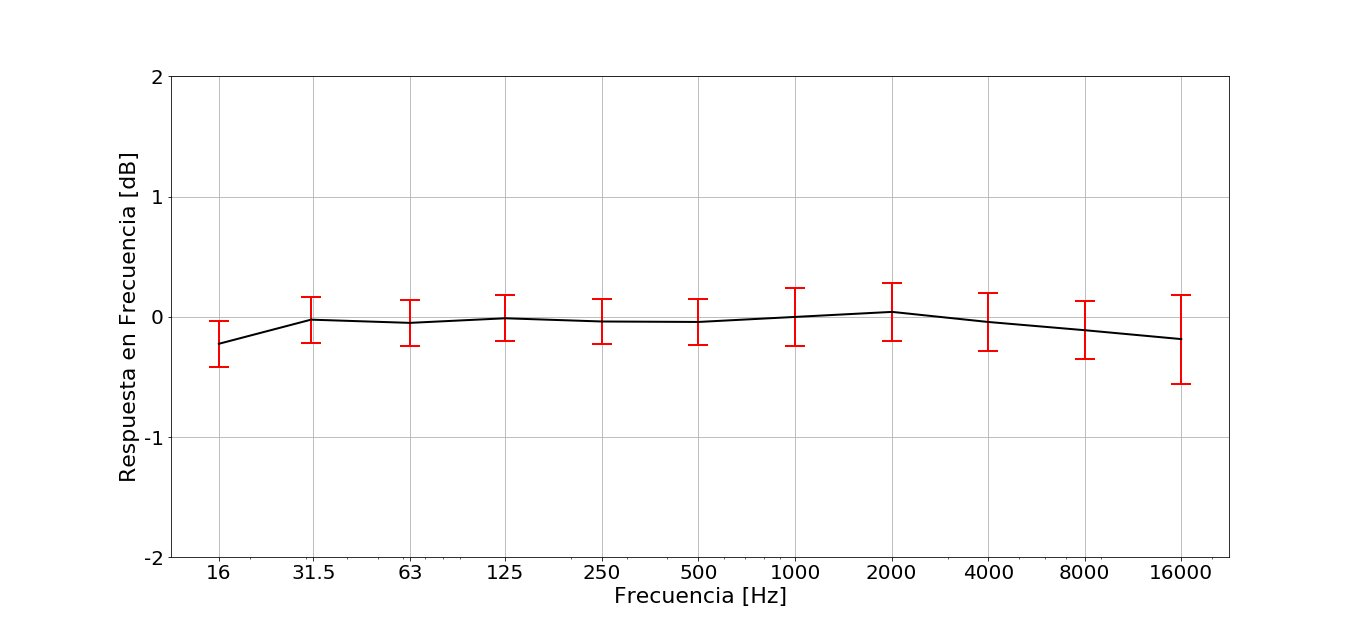
\includegraphics[width=15.5 cm]{RespFrec.jpg}
	\caption[RespFrec]{Respuesta en frecuencia del amplificador en condición estándar.} 
	\label{fig:RespFrec}
\end{figure}

En la Tabla \ref{tab:FrecRang} se expresan los resultados del ancho de frecuencia limitado por ganancia. Cabe destacar que la frecuencia de corte inferior se vio limitada por la menor frecuencia que se pudo generar con el generador de señales utilizado, con lo que la atenuación de 3 dB no fue alcanzada.


\begin{table}[h]
	\centering
	\caption{Resultados de la medición de respuesta en frecuencia (k = 2).}
	\begin{tabular}{cccc}
		\hline
		\textbf{Frecuencia}&\textbf{$V_{in}$}&\textbf{$V_{out}$}&\textbf{Atenuación}\\\hline
		
		1000,12 Hz ± 0,07 Hz & 448,44 mV ± 0,67 mV & 22,596 V ± 0,06 V &       0 dB \\\hline
		
		9,622 Hz ± 0,01 Hz & 445,53 mV ± 2,26 mV & 18,126 V ± 0,08 V & 1,915 dB  ± 0,002 dB \\\hline
		
		90619,2 Hz ± 6,28 Hz & 453,05 mV ± 4,72 mV & 15,927 V ± 0,12 V & 3,038 dB  ± 0,003 dB \\\hline
		
	\end{tabular}  
	\label{tab:FrecRang}
\end{table}

\subsection{Diseño prueba objetiva: Definición de Variables.}
Lorem ipsum dolor sit amet consectetur adipiscing, elit cum ultricies inceptos tortor auctor, eros velit neque sollicitudin hac. Blandit accumsan felis dictumst phasellus vivamus integer pharetra egestas euismod hendrerit, porta faucibus turpis cubilia urna mauris luctus erat ut, facilisis dis velit natoque tempor libero potenti gravida lectus. Nisl mollis ultricies imperdiet justo per blandit purus fames, duis montes condimentum sodales tristique a torquent porta elementum, nisi convallis ante id rutrum netus nibh.

\subsection{Diseño prueba subjetiva: Encuesta y Muestra.}
Lorem ipsum dolor sit amet consectetur adipiscing, elit cum ultricies inceptos tortor auctor, eros velit neque sollicitudin hac. Blandit accumsan felis dictumst phasellus vivamus integer pharetra egestas euismod hendrerit, porta faucibus turpis cubilia urna mauris luctus erat ut, facilisis dis velit natoque tempor libero potenti gravida lectus. Nisl mollis ultricies imperdiet justo per blandit purus fames, duis montes condimentum sodales tristique a torquent porta elementum, nisi convallis ante id rutrum netus nibh. 


\section{Validación de las pruebas.}
Lorem ipsum dolor sit amet consectetur adipiscing, elit cum ultricies inceptos tortor auctor, eros velit neque sollicitudin hac. Blandit accumsan felis dictumst phasellus vivamus integer pharetra egestas euismod hendrerit, porta faucibus turpis cubilia urna mauris luctus erat ut, facilisis dis velit natoque tempor libero potenti gravida lectus. Nisl mollis ultricies imperdiet justo per blandit purus fames, duis montes condimentum sodales tristique a torquent porta elementum, nisi convallis ante id rutrum netus nibh.
\section{Análisis de los resultados: Aplicaciones estadísticas.}
Lorem ipsum dolor sit amet consectetur adipiscing, elit cum ultricies inceptos tortor auctor, eros velit neque sollicitudin hac. Blandit accumsan felis dictumst phasellus vivamus integer pharetra egestas euismod hendrerit, porta faucibus turpis cubilia urna mauris luctus erat ut, facilisis dis velit natoque tempor libero potenti gravida lectus. Nisl mollis ultricies imperdiet justo per blandit purus fames, duis montes condimentum sodales tristique a torquent porta elementum, nisi convallis ante id rutrum netus nibh.
\section{Conclusiones}
Lorem ipsum dolor sit amet consectetur adipiscing, elit cum ultricies inceptos tortor auctor, eros velit neque sollicitudin hac. Blandit accumsan felis dictumst phasellus vivamus integer pharetra egestas euismod hendrerit, porta faucibus turpis cubilia urna mauris luctus erat ut, facilisis dis velit natoque tempor libero potenti gravida lectus. Nisl mollis ultricies imperdiet justo per blandit purus fames, duis montes condimentum sodales tristique a torquent porta elementum, nisi convallis ante id rutrum netus nibh.
\section{Líneas futuras de investigación.}
Lorem ipsum dolor sit amet consectetur adipiscing, elit cum ultricies inceptos tortor auctor, eros velit neque sollicitudin hac. Blandit accumsan felis dictumst phasellus vivamus integer pharetra egestas euismod hendrerit, porta faucibus turpis cubilia urna mauris luctus erat ut, facilisis dis velit natoque tempor libero potenti gravida lectus. Nisl mollis ultricies imperdiet justo per blandit purus fames, duis montes condimentum sodales tristique a torquent porta elementum, nisi convallis ante id rutrum netus nibh.
\section{Cronograma}

\section{Bibliografía}
\printbibliography[heading=none]

\end{document}